\documentclass{article}
\usepackage{amsmath,amssymb}
\usepackage{tikz}
\usetikzlibrary{arrows.meta,positioning,calc,shapes.geometric}
\pagestyle{empty}
\begin{document}
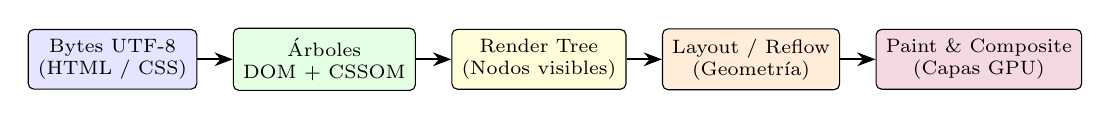
\begin{tikzpicture}
\tikzset{node distance=0.45cm, every node/.style={font=\scriptsize, draw, rounded corners=2pt, align=center, inner sep=3.5pt}}
\node (bytes) [fill=blue!10] {Bytes UTF-8\\(HTML / CSS)};
\node (dom) [right=of bytes, fill=green!10] {Árboles\\DOM + CSSOM};
\node (render) [right=of dom, fill=yellow!15] {Render Tree\\(Nodos visibles)};
\node (layout) [right=of render, fill=orange!15] {Layout / Reflow\\(Geometría)};
\node (paint) [right=of layout, fill=purple!15] {Paint \& Composite\\(Capas GPU)};
\draw[-Stealth, thick] (bytes) -- (dom);
\draw[-Stealth, thick] (dom) -- (render);
\draw[-Stealth, thick] (render) -- (layout);
\draw[-Stealth, thick] (layout) -- (paint);
\end{tikzpicture}
\end{document}
